% !TEX encoding = UTF-8 Unicode
% J.Roussel
% MAJ : 2014-06-03
%-------------------------------------------
\documentclass[11pt]{article}
\input{styles_meca}
\title{Figures TIKZ du cours sur les oscillateurs}
\begin{document}
	
%------ oscillations harmoniques------
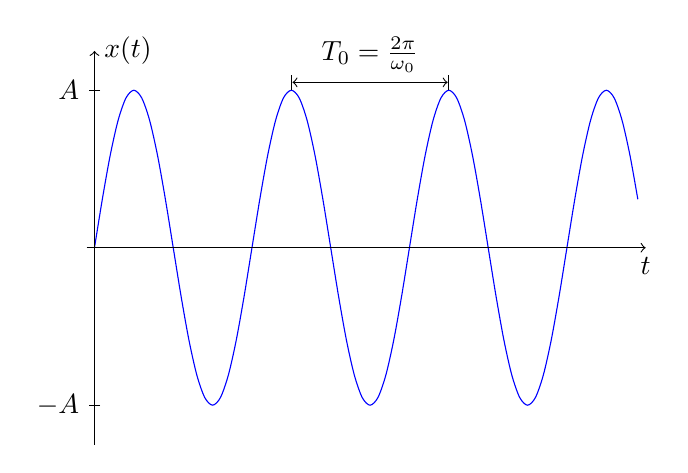
\begin{tikzpicture}[scale=1]
	\def \xLabel {$t$}; % legende sur x
    \def \yLabel {$x(t)$}; % legende sur y
    \def \xmin{-0.1}; 
    \def \xmax{7};
    \def \ymin{-2.5};
    \def \ymax{2.5};
    \draw[smooth,color=blue, variable=\x, samples at={0,0.1,...,7}]   plot (\x,{2*sin(\x r*pi)}) ;
    \draw[->] (\xmin,0) -- (\xmax,0) node[below] {\xLabel};
    \draw[->] (0,\ymin) -- (0,\ymax) node[right] {\yLabel};
    \foreach \y/\ytext in {-2/-A,2/A} 
    \draw[shift={(0,\y)}] (2pt,0pt) -- (-2pt,0pt) node[left] {$\ytext$};  
    \draw[|<->|] (2.5,2.1)--++(2,0) node[pos=0.5, above]{$T_{0}=\frac{2\pi}{\omega_{0}}$};
\end{tikzpicture}
%============================================================
% 	Sujet : Représentation des oscillations en régime pseudo-périodique d'un 
%	pendule élastique ainsi que de l'évolution de son énergie mécanique. 
%	On a choisit une masse $m=[1]{kg}$,  une de pulsation propre $\omega_{0}=[1]{rad.s^{-1}}$
%	 et un facteur de qualité $Q=10$. Les conditions initiales sont $x(0)=0$ et $\dot x(0)=[1,5]{SI}$.
%============================================================                   

\begin{tikzpicture}
\begin{axis}[
	name=plot1,
	height=7cm,
	width=7cm,
	axis lines=middle,% bottom,top
	inner axis line style={=>},
	xlabel={$t$ (s)},
	ylabel={$x$},
	xtick={1,2,3,4},
	xticklabels={10,20,30,40},
	ytick={-1,1},
	yticklabels={-1,1},
	ymin=-2,
	ymax=2,
	xmin=0,
	xmax=4.8,]
	\addplot+[mark=none] table[x index=0,y index=1]{simu/rk4harmonique-xt-Q10.txt};
	\addplot+[mark=none,color=gray,domain=0:4,samples=100]{1.77*exp(-0.51*x)};
	\addplot+[mark=none,color=gray,domain=0:4,samples=100]{-1.77*exp(-0.51*x)};
\end{axis}
\begin{axis}[
	name=plot2,
	at={($(plot1.east)+(1cm,0)$)},
	anchor=west,
	height=7cm,
	width=7cm,
	axis lines=middle,% bottom,top
	inner axis line style={=>},
	xlabel={$t$ (s)},
	ylabel={$E_{\rm m}=\frac{1}{2}kx^{2}+\frac{1}{2}mv^{2}$},
	xtick={1,2,3,4},
	xticklabels={10,20,30,40},
	ytick={4},
	yticklabels={1},
	ymin=0,
	ymax=4.4,
	xmin=0,
	xmax=4.8,]
	\addplot+[mark=none] table[x index=0,y index=1]{simu/rk4harmonique-Et-Q10.txt};
\end{axis}
\end{tikzpicture}
%============================================================
%	Représentation des oscillations en régime apériodique d'un pendule élastique 
%	ainsi que de l'évolution de son énergie mécanique. On a choisit une masse 
%	$m=[1]{kg}$,  une de pulsation propre $\omega_{0}=[1]{rad.s^{-1}}$ et un facteur 
%	de qualité $Q=\frac{1}{10}$. Les conditions initiales sont $x(0)=0$ et $\dot x(0)=[1,5]{SI}$.
%============================================================          
\begin{tikzpicture}
\begin{axis}[
	name=plot1,
	height=7cm,
	width=7cm,
	axis lines=middle,% bottom,top
	inner axis line style={=>},
	xlabel={$t$ (s)},
	ylabel={$x$},
	xtick={2,4},
	xticklabels={10,20},
	ytick={2},
	yticklabels={$10^{-1}$},
	ymin=0,
	ymax=4,
	xmin=0,
	xmax=4.8,]
	\addplot+[mark=none] table[x index=0,y index=1]{simu/rk4harmonique-xt-aperiodique.txt};
\end{axis}
\begin{axis}[
	name=plot2,
	at={($(plot1.east)+(1cm,0)$)},
	anchor=west,
	height=7cm,
	width=7cm,
	axis lines=middle,% bottom,top
	inner axis line style={=>},
	xlabel={$t$ (s)},
	ylabel={$E_{\rm m}=\frac{1}{2}kx^{2}+\frac{1}{2}mv^{2}$},
	xtick={0.8,1.6,2.4,3.2,4},
	xticklabels={2,4,6,8,10},
	ytick={2},
	yticklabels={$10^{-1}$},
	ymin=0,
	ymax=4,
	xmin=0,
	xmax=4.8,]
	\addplot+[mark=none] table[x index=0,y index=1]{simu/rk4harmonique-Et-aperiodique.txt};
\end{axis}
\end{tikzpicture}

%============================================================
% 	Représentation des oscillations en régime critique d'un pendule élastique 
%	ainsi que de l'évolution de son énergie mécanique. On a choisit une masse 
%	$m=[1]{kg}$,  une de pulsation propre $\omega_{0}=[1]{rad.s^{-1}}$ et un 
%	facteur de qualité $Q=0,5$. Les conditions initiales sont $x(0)=0$ et $\dot x(0)=[1,5]{SI}$.
%============================================================        
\begin{tikzpicture}
\begin{axis}[
	name=plot1,
	height=7cm,
	width=7cm,
	axis lines=middle,% bottom,top
	inner axis line style={=>},
	xlabel={$t$ (s)},
	ylabel={$x$},
	xtick={1,2,3,4},
	xticklabels={10,20,30,40},
	ytick={2},
	yticklabels={0.5},
	ymin=0,
	ymax=4,
	xmin=0,
	xmax=4.8,]
	\addplot+[mark=none] table[x index=0,y index=1]{simu/rk4harmonique-xt-critique.txt};
\end{axis}
\begin{axis}[
	name=plot2,
	at={($(plot1.east)+(1cm,0)$)},
	anchor=west,
	height=7cm,
	width=7cm,
	axis lines=middle,% bottom,top
	inner axis line style={=>},
	xlabel={$t$ (s)},
	ylabel={$E_{\rm m}=\frac{1}{2}kx^{2}+\frac{1}{2}mv^{2}$},
	xtick={1,2,3,4},
	xticklabels={10,20,30,40},
	ytick={4},
	yticklabels={1},
	ymin=0,
	ymax=4,
	xmin=0,
	xmax=4.8,]
	\addplot+[mark=none] table[x index=0,y index=1]{simu/rk4harmonique-Et-critique.txt};
\end{axis}
\end{tikzpicture}
%============================================================
%	Date : 21 Oct. 2010		Sujjet : pendule élastique
%============================================================
\begin{tikzpicture} [scale=1, decoration={coil,aspect=0.3,segment length=3mm,amplitude=3mm},  ressort/.style={thick,black,smooth,}]
\colorlet{darkblue}{blue!50!black};  
\draw[bloc] (4,-0.5) rectangle (5,0.5);
\draw (0,0)--(0.5,0);
\draw[ressort,decorate] (0.5,0)--(4,0) ;
\fill [pattern=north east lines] (6,-0.5)--++(-6,0)--++(0,1)--++(-0.3,0)--++(0,-1.3)--++(6.3,0)-- cycle;
\draw[thick,color=gray](6,-0.5)--++(-6,0)--++(0,1);
\draw[force] (4,0) --++(-2,0) node[midway, above=3mm]{$\overrightarrow{T}$};
\draw[color=gray] (0,0.75)--++(0,0.5);
\draw[->,color=gray] (0,0.9)--++(2,0) node[pos=0.4,fill=white]{$\ell_{0}$};
\draw[->,color=gray] (0,1.1)--++(4,0) node[pos=0.7,fill=white]{$\ell_{0}+x$};
\end{tikzpicture}
%============================================================
%	Date : 21 Oct. 2010		Sujjet : pendule élastique en régime forcé
%============================================================

\begin{tikzpicture}[scale=1.2, decoration={coil,aspect=0.3,segment length=3mm,amplitude=3mm},  ressort/.style=
 {thick,gray,smooth,}]
\draw[bloc] (4,-0.5) rectangle (5,0.5);
\draw[ressort,decorate] (0.5,0)--(4,0) ;
\fill [pattern=north east lines] (6,-0.5)--++(-8,0)--++(0,-0.3)--++(8,0)-- cycle;
\draw[thick,color=gray](6,-0.5)--++(-8,0);
\draw[thin,color=gray] (-1,-0.5)--++(0,1);
\draw[color=gray] (0,0)--++(0,1);
\draw[->,color=gray] (0,0.75)--++(4,0) node[pos=0.4,fill=white]{$\ell(t)$};
\draw[->,color=gray] (-1,0.5)--++(1,0) node[above left]{\small $a\cos\omega t$};
\draw[force](0,0)--++(-1.2,0)node[left]{$\overrightarrow{f}_{\!\!\textrm{op}}$};
\draw[force](0,0)--++(1.2,0)node[right,fill=white]{$\overrightarrow{T'}$};
\draw (0,0)node{$\bullet$}node[below=5pt]{E}--(0.5,0);
\end{tikzpicture}

%============================================================
%	 Potentiel de Lenard-Jones modélisant l'interaction entre deux atomes. 
%	Le puits de potentiel peut s'approcher au voisinage du minimum, par une approximation harmonique.
%============================================================   
 \begin{tikzpicture}[scale=2]
	\def \xLabel {$x$}; 
        \def \yLabel {$E_{\rm p}$}; 
        \def \xmin{1}; 
        \def \xmax{4.5};
        \def \ymin{-1};
        \def \ymax{2}; 
          \draw[color=blue]  plot  file {simu/lennard-jones.txt} ;
           \draw[smooth,color=gray, variable=\x, samples at={0.75,0.85,...,1.3}]   plot ({2*\x},{36*(\x-1)^2-1});
        	\draw[->] (\xmin,0) -- (\xmax,0) node[below] {\xLabel};
        \draw[->] (\xmin,\ymin) -- (\xmin,\ymax) node[below right] {\yLabel};
        \draw (2.6,1) node[right]{$E_{\rm p}=E_{\rm p,min}+\frac{1}{2}k(x-x_{\rm eq})^{2}$};
 \end{tikzpicture}
 
% approximation harmonique du pendule simple
\begin{tikzpicture} [scale=0.8]
\begin{scope}
\coordinate (O) at (0, 0);
\coordinate (M) at (-55:5);
\draw[thick] (O)--(M); 
\draw[thick,->] (0,-1.2) arc(-90:-55:1.2) ;
\draw (-90:1.5) node[right]{$\theta(t)$} (-57:2.5) node[above right]{$\ell$};
\draw[vecteur] (M)--++({cos(55)},{-sin(55)}) node[below right ]{$\overrightarrow{u_r}$};
\draw[vecteur] (M)--++({sin(55)},{cos(55)}) node[above right ]{$\overrightarrow{u_{\theta}}$};
\draw[force] (M)--(-55:3) node[below left]{$\overrightarrow{T}$};
\draw[force] (M)--++(0,-2) node[right]{$\overrightarrow{P}=m \overrightarrow{g}$};
\draw[bloc] (M) circle(0.15) node[black,right=5pt]{M($\ell$,$\theta$)};
\draw [ultra thick,gray] (-1,0)--(1,0); 
\draw [thin,gray]  (0,0.5) --(0,-6);   
\draw[vecteur] (-1,-1)--++(0,-1) node[midway,right]{$\overrightarrow{g}$};
\end{scope}
\begin{scope}[xshift=9cm,yshift=-3cm]
\def \xLabel {$\theta$}; % legende sur x
\def \yLabel {$E_{\rm p}$}; % legende sur y
\def \xmin{-3.5}; 
\def \xmax{3.5};
\def \ymin{-3};
\def \ymax{3};
\def \stepGrid{0.5cm}; % pas de la grille
\def \titleWidth {7cm}; % largeur de la vignette de titre
\draw[->] (\xmin,0) -- (\xmax,0) node[above=2pt] {\xLabel};
\draw[->] (0,\ymin) -- (0,\ymax) node[below right] {\yLabel};
\draw[style=help lines,step=\stepGrid,color=gray,opacity=0.5] (\xmin,\ymin) grid (\xmax,\ymax);
\foreach \x/\xtext in {-pi/-\pi,pi/\pi}
	\draw[shift={(\x,0)}] (0pt,2pt) -- (0pt,-2pt) node[below] {$\xtext$};
\foreach \y/\ytext in {-2/-mg\ell,2/mg\ell}
	\draw[shift={(0,\y)}] (2pt,0pt) -- (-2pt,0pt) node[left] {$\ytext$};
\draw[thick,color=blue, variable=\x, samples at={\xmin,-3.4,...,\xmax}] plot ({\x}, {-2*cos(\x r)}) ;
\draw[thick,color=purple, variable=\x, samples at={-1.9,-1.8,...,1.9}] plot ({\x}, {\x*\x-2}) ;
\draw[purple] (1.6,2.5) --++(0.5,0) node[text width=2cm, right,black]{\small approximation harmonique};
\end{scope}
\end{tikzpicture} 
 

 
 %------ Réponse fréquentielle de l'amplitude d'un oscillateur vis à vis d'une excitation sinusoïdale.
 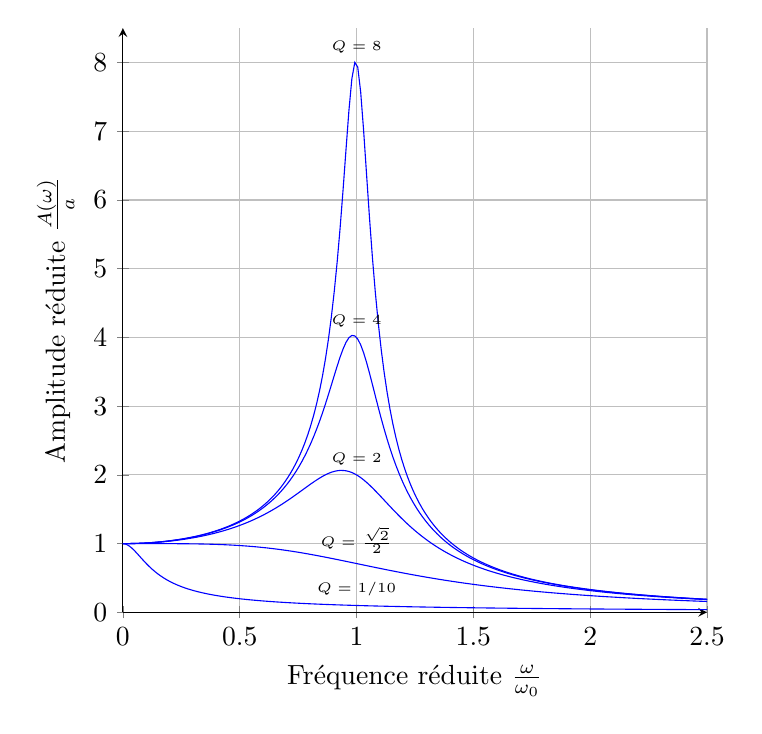
\begin{tikzpicture}[scale=1]
 	\def \xLabel {Fréquence réduite $\frac{\omega}{\omega_{0}}$};
 	\def \yLabel {Amplitude réduite $\frac{A(\omega)}{a}$}; 
 	\def \xMin{0}; 
 	\def \xMax{2.5};
 	\def \yMin{0};
 	\def \yMax{8.5};
 	\begin{axis}[width=9cm,height=9cm,xlabel={\xLabel},ylabel={\yLabel},%grid=major,
 	grid=both,
 	axis x line=bottom,axis y line=left,%enlarge x limits=false,
 	try min ticks=2,
 	xmin=\xMin,xmax=\xMax,ymin=\yMin,ymax=\yMax,]
 	\foreach \facteurQ in {0.1,0.71,2,4,8}  
              {
              \addplot+[mark=none,color=blue,domain=\xMin:\xMax,samples=200]{1/sqrt((1-x*x)*(1-x*x)+(x/\facteurQ)*(x/
              \facteurQ))};
             }
          \draw (axis cs:1,0.1) node[ above]{\tiny $Q=1/10$};
          \draw (axis cs:1,0.707) node[above]{\tiny $Q=\frac{\sqrt{2}}{2}$};
          \draw (axis cs:1,2) node[above]{\tiny $Q=2$};
          \draw (axis cs:1,4) node[above]{\tiny $Q=4$};
          \draw (axis cs:1,8) node[above]{\tiny $Q=8$};
         \end{axis}
         \end{tikzpicture}

%------ Évolution de l'amplitude de la vitesse en fonction de la fréquence pour différentes valeur du facteur de qualité.
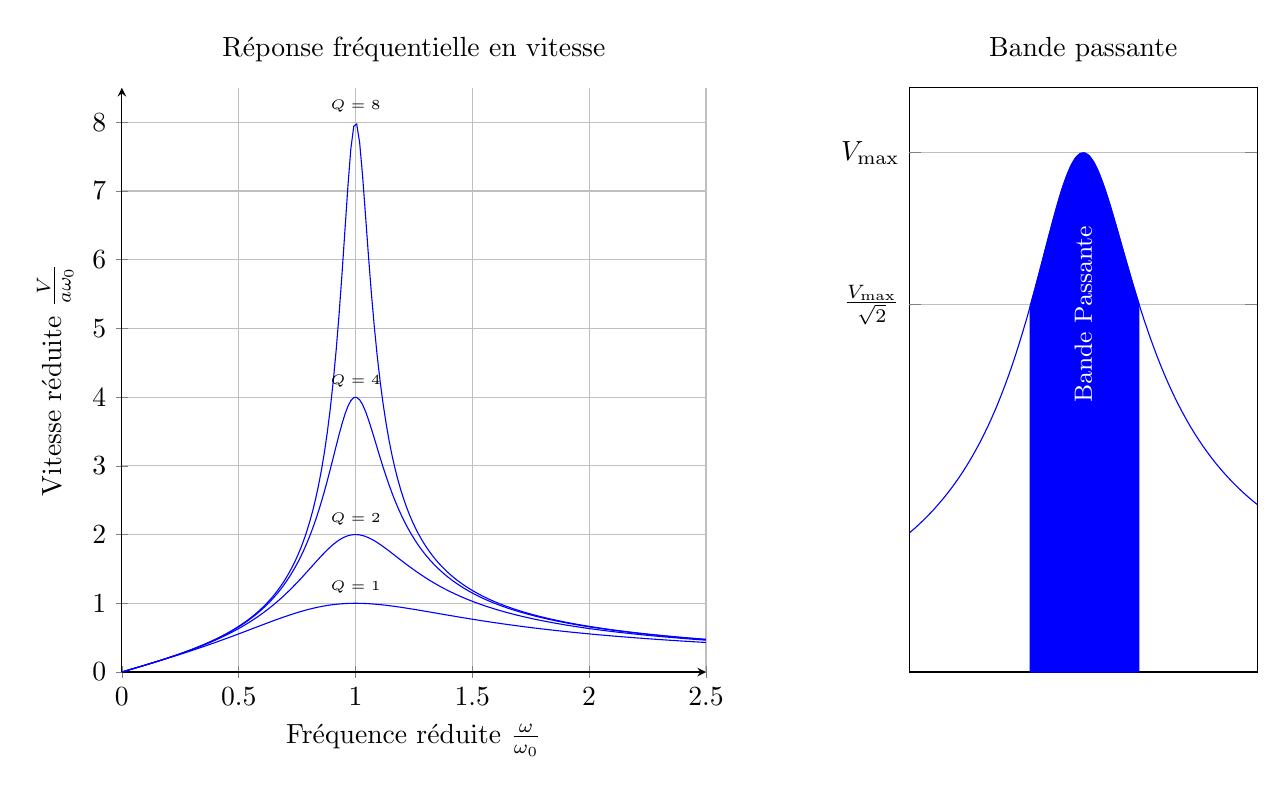
\begin{tikzpicture}[scale=1]
	\begin{scope}
	\begin{axis}[
		width=9cm,
		height=9cm,
		title={Réponse fréquentielle en vitesse},
		xlabel={Fréquence réduite $\frac{\omega}{\omega_{0}}$},
		ylabel={Vitesse réduite $\frac{V}{a\omega_{0}}$},
		%grid=major,
		grid=both,
		axis x line=bottom,
		axis y line=left,%enlarge x limits=false,
		try min ticks=2,
		xmin=0,
		xmax=2.5,
		ymin=0,
		ymax=8.5]
		\foreach \facteurQ in {1,2,4,8}
		{\addplot+[mark=none,color=blue,domain=0:2.5,samples=200]{\facteurQ/sqrt(1+(\facteurQ*(1/x-x))*(\facteurQ*(1/x-x)))};}
         \draw (axis cs:1,1) node[above]{\tiny $Q=1$};
         \draw (axis cs:1,2) node[above]{\tiny $Q=2$};
         \draw (axis cs:1,4) node[above]{\tiny $Q=4$};
         \draw (axis cs:1,8) node[above]{\tiny $Q=8$};
        \end{axis}
        \end{scope}
        \begin{scope}[xshift=10cm]
        \begin{axis}[
			width=6cm,
			height=9cm,	
			grid=none,
			title={Bande passante},
			enlarge x limits=false,
			xmin=0.8,
			xmax=1.2,
			ymin=0,
			ymax=9,
			xtick=\empty,
			ytick=\empty,
			extra y ticks={8,5.66},
			extra y tick labels={$V_{\rm max}$,$\frac{V_{\rm max}}{\sqrt{2}}$}, 
			extra y tick style={grid=major},]
			\addplot+[mark=none,color=blue,domain=0.8:1.2,samples=200]{8/sqrt(1+(8*(1/x-x))*(8*(1/x-x)))};
			\addplot+[mark=none,color=blue,fill,domain=0.939:1.064]{8/sqrt(1+(8*(1/x-x))*(8*(1/x-x)))} \closedcycle;
			\draw (axis cs:1,4) node[rotate=90,right,color=white] {\small Bande Passante}; 
         \end{axis}
        \end{scope} 
\end{tikzpicture}

%============================================================
%	 Réponse fréquentielle de la vitesse d'un oscillateur vis à vis d'une excitation sinusoïdale.
%============================================================   
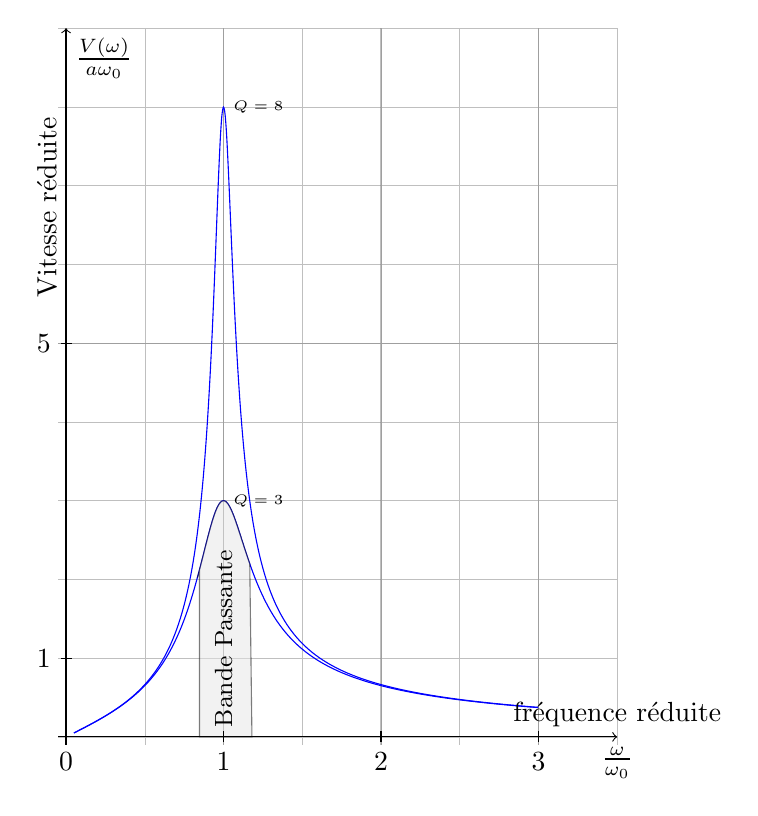
\begin{tikzpicture}[scale=1]
	\def \xLabel {$\frac{\omega}{\omega_{0}}$}; 
        \def \yLabel {$\frac{V(\omega)}{a\omega_{0}}$}; 
        \def \xmin{-0.1}; 
        \def \xmax{7};
        \def \ymin{-0.1};
        \def \ymax{9};     
        \draw[color=gray,opacity=0.5] (\xmin,\ymin) grid[xstep=2, ystep=5] (\xmax,\ymax);
        \draw[very thin,color=gray,opacity=0.5] (\xmin,\ymin) grid[xstep=1, ystep=1] (\xmax,\ymax);
        \foreach \facteurQ/\color in {3/red,8/blue}  
        {\draw[smooth,color=blue,\color, variable=\x, samples at={0.05,0.06,...,3}]   plot ({2*\x},{1/sqrt(1/(\facteurQ*\facteurQ)+(\x-1/\x)*(\x-1/\x))}) ;
        \draw (2,\facteurQ) node[right]{\tiny $Q=\facteurQ$};
         }
        \fill[fill=gray!20,draw=black,opacity=0.5] ({(-1+sqrt(37))/3},0) --++(0,{1.5*sqrt(2)}) -- plot[domain={5/6}:{7/6}] ({2*\x},{1/sqrt(1/9+(\x-1/\x)*(\x-1/\x))})  -- ({(1+sqrt(37))/3},0) -- cycle;
	\draw[->] (\xmin,0) -- (\xmax,0) node[below] {\xLabel} node[above]{fr\'equence r\'eduite};
        \draw[->] (0,\ymin) -- (0,\ymax) node[below right] {\yLabel} node[above,pos=0.75,rotate=90]{Vitesse r\'eduite };
        \foreach \x in {0,1,2,3}
        \draw[shift={(2*\x,0)}] (0pt,2pt) -- (0pt,-2pt) node[below] {$\x$};
        \foreach \y in {1,5} 
        \draw[shift={(0,\y)}] (2pt,0pt) -- (-2pt,0pt) node[left] {$\y$}; 
          \draw (2,0) node[rotate=90,right] {\small Bande Passante}; 
 \end{tikzpicture}
 
%==========================================================
% Pendule simple : évolution de sa période T en unité de $T_{0}$ (période dans l'approximation harmonique)
% en fonction de l'amplitude des oscillations.
%=========================================================
\begin{tikzpicture}[scale=1]
\begin{axis}[
	xlabel={angle $\theta_{\textrm{max}}$ (°)},
	ylabel={$T/T_{0}$},
	extra x ticks={180}, 
	extra x tick labels={180}, 
	extra x tick style={grid=major},
	grid=major,
	axis x line=bottom,
	axis y line=left,
	xmin=0,
	xmax=190,
	ymin=0,
	ymax=3.9,
	]
	\addplot+[mark=none] table[x=angle,y=T]{simu/periodes-pendule.txt};
\end{axis}
\end{tikzpicture}

% ===========================================================
%  Date :2013-09-05 		sujet : oscillateur harmonique pour Pierre
% ===========================================================


\begin{tikzpicture} [scale=1.5, decoration={coil,aspect=0.3,segment length=3mm,amplitude=3mm},  ressort/.style=
{thick,black,smooth,}]
\draw[bloc] (4,-0.5) rectangle (5,0.5);
\draw (0,0)--(0.5,0);
\draw[ressort,decorate] (0.5,0)--(4,0) ;
\fill [pattern=north east lines] (6,-0.5)--++(-6,0)--++(0,1)--++(-0.3,0)--++(0,-1.3)--++(6.3,0)-- cycle;
\draw[thick,color=gray](6,-0.5)--++(-6,0)--++(0,1);
\draw[force] (4,0) --++(-2,0) node[midway, above=3mm]{$\overrightarrow{T}$};
\draw[force] (4.5,-0.5) --++(-1,0) node[left]{$\overrightarrow{f}$};
\draw[color=gray] (0,0.75)--++(0,0.5);
\draw[->,color=gray] (0,0.9)--++(2,0) node[pos=0.4,fill=white]{$\ell_{0}$};
\draw[->,color=gray] (0,1.1)--++(4,0) node[pos=0.7,fill=white]{$\ell_{0}+x$};
\end{tikzpicture}

% Potentiel de Morse
\begin{tikzpicture}[scale=1]
  \begin{axis}[
	  title={Morse : $E_{p}=E_{0}\left(\mathrm{e}^{-2ax}-2\mathrm{e}^{-ax}\right)$ },
	  xtick=\empty,
	  extra y ticks={-1,0},
	  extra y tick labels={$-E_{0}$,0},
	  extra y tick style={grid=major},
	  ytick=\empty,
	  extra x ticks={0}, 
	  extra x tick labels={0}, 
	  extra x tick style={grid=major},
	  xlabel={écart à l'équilibre $x$}, 
	  ylabel={$E_{\textrm{p}}$},
	  xmin=-0.5,
	  xmax=1,
	  ymin=-1.5,
	  ymax=4]
 \addplot+[mark=none]table[x=x,y=Morse]{simu/potentiels-anharmoniques.txt};
 \end{axis}
\end{tikzpicture}

% ==============================================================
% Date : 2014-08-01
% Solution $x(t)$ de l'oscillateur de Duffing avec $A=1$ et  $\omega_{0}=1$.
% Comparaison entre la solution approximative \ref{eq:C6DuffingLindstedt} et la solution
% numérique obtenue par la méthode d'Euler.
% ==============================================================
\begin{tikzpicture}[scale=1]
\begin{scope}
\begin{axis}[
	 title={Oscillateur de Duffing : $\epsilon=0,1$},
	 xlabel={temps},
	 grid=major,
	 axis x line=bottom,
	 axis y line=left,
	 xmin=0,
	 xmax=20,
	 ymin=-1.5,
	 ymax=1.3,
	 legend style = {at={(0.5,0.02)},anchor=south},legend columns=2]
	 \addplot+[mark=none,dashed] table[x=temps,y=x]{simu/oscillateurDuffing0.1.txt};
	 \addlegendentry{\small Euler };
	 \addplot+[mark=none] table[x=temps,y=approxLindstedt]{simu/oscillateurDuffing0.1.txt};
	 \addlegendentry{\small Lindstedt (ordre un) };
\end{axis}
\end{scope}
\begin{scope}[xshift=8cm]
 \begin{axis}[
	 title={Oscillateur de Duffing : $\epsilon=1$},
	 xlabel={temps},
	 grid=major,
	 axis x line=bottom,
	 axis y line=left,
	 xmin=0,
	 xmax=20,
	 ymin=-1.5,
	 ymax=1.3,
	 legend style = {at={(0.5,0.02)},anchor=south},legend columns=2]
	 \addplot+[mark=none,dashed] table[x=temps,y=x]{simu/oscillateurDuffing1.txt};
	 \addlegendentry{\small Euler };
	 \addplot+[mark=none] table[x=temps,y=approxLindstedt]{simu/oscillateurDuffing1.txt};
	 \addlegendentry{\small Lindstedt (ordre un)};
 \end{axis}
 \end{scope}
\end{tikzpicture}


\end{document}